% Schematic of the step limit: the Jacobian determinant at one quadrature point along the Newton
% step, det(J0 - lambda dJ), a polynomial in lambda. The curve is illustrative, not simulation data.
\begin{figure}[htbp]
    \centering
    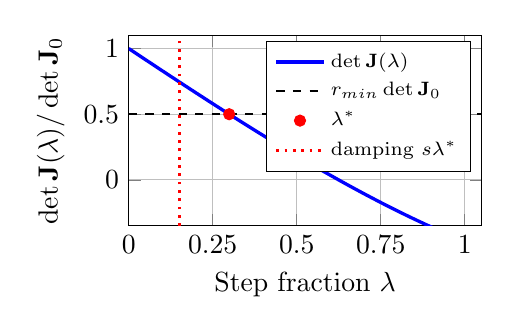
\begin{tikzpicture}
        \begin{axis}[
                width=0.5\linewidth,
                height=0.33\linewidth,
                xmin=0, xmax=1.05,
                ymin=-0.35, ymax=1.1,
                xlabel={Step fraction $\lambda$},
                ylabel={$\det\mathbf{J}(\lambda)/\det\mathbf{J}_0$},
                xtick={0,0.25,0.5,0.75,1},
                legend pos=north east,
                legend cell align=left,
                legend style={font=\scriptsize},
                grid=major,
            ]
            \addplot[blue, line width=1.2pt, domain=0:1, samples=200] {(1-1.6*x)*(1-0.4*x)*(1+0.3*x)};
            \addlegendentry{$\det\mathbf{J}(\lambda)$}
            \addplot[black, dashed, line width=0.8pt, domain=0:1.05] {0.5};
            \addlegendentry{$r_\text{min}\det\mathbf{J}_0$}
            \addplot[red, only marks, mark=*, mark size=2pt] coordinates {(0.299,0.5)};
            \addlegendentry{$\lambda^\ast$}
            \addplot[red, dotted, line width=1pt] coordinates {(0.15,-0.35) (0.15,1.1)};
            \addlegendentry{damping $s\lambda^\ast$}
        \end{axis}
    \end{tikzpicture}
    \caption{Schematic of the step limit at one quadrature point. The determinant of the element map is a polynomial in the step fraction $\lambda$. The damper finds the first $\lambda^\ast$ at which it drops to $r_\text{min}$ times its current value, and the Newton step is scaled to $s\lambda^\ast$ (here $s=r_\text{min}=0.5$; the curve is illustrative).}\label{fig:damper_schematic}
\end{figure}
